\documentclass[12pt,titlepage]{article}

\usepackage{geometry}
\geometry{
    a4paper,
    left=3cm,
    right=2.5cm,
    top=2.5cm,
    bottom=2.5cm
}
\usepackage{graphicx}
\usepackage{caption}
\usepackage{hyperref}

\title{
    Further Topics and Goodbye!
    \vspace{2cm}
    \begin{figure}[h]
        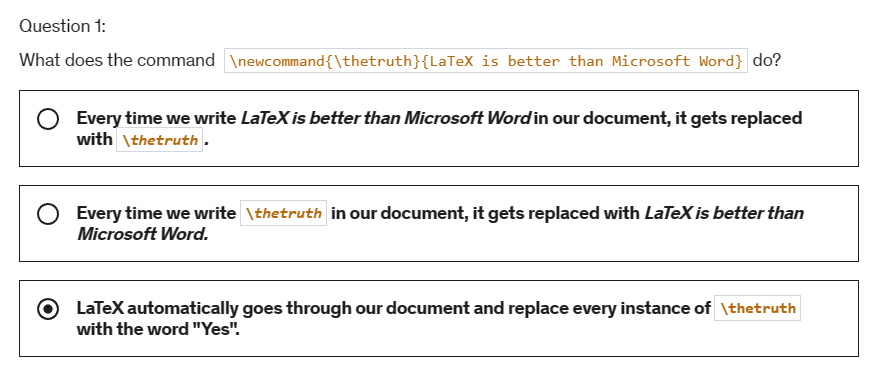
\includegraphics[width = \linewidth]{../Screenshot_1.png}
        \caption*{The grand truth}
    \end{figure}
}
\author{Me}
\date{\today}

\begin{document}
\maketitle

\newpage
\thispagestyle{empty}
\tableofcontents
\newpage

\section{Displaying Code with Verbatim (YIKES...)}
\url{https://www.overleaf.com/learn/latex/Code_listing}

We can use either the inline \verb?\verb|text|? environment or "block"
\begin{verbatim}
    \begin{verbatim }
    \end{verbatim }
\end{verbatim}

\section{Multiple Files}
\begin{verbatim}
\usepackage{subfiles}

\subfile{Section1}

In the Section1.tex we srite:
\documentclass[main.tex]{subfiles}

\begin{document}
\section{Section 1}
It is the section inside of the subfile.
\end{document}
\end{verbatim}

\section{Custom Commands}
\begin{verbatim}
We can create new commands in the preamble of the document:
    \newcommand{\intinf}{\int_{1}^{\infty}}
Now when we write the \intinf we se the entire integral with proper limits.

Or to have a proper spacing when usin abbreviations ending with a period:
    \newcommand{\eg}{e.g.\ }
    \newcommand{\ie}{i.e.\ }
\end{verbatim}

\subsection{Arguments in Custom Commands}

\url{https://www.overleaf.com/learn/latex/Commands}

\begin{verbatim}
We specify the number of inputs in the [] and then use a #1 which is
the number of the input given to the command.
    \newcommand{\intinf}[1]{\int_{#1}^{\infty}}
\end{verbatim}

\section{Resources and Goodbye!}
\begin{itemize}
    \item \url{https://no.overleaf.com/learn}
    \item \url{https://en.wikibooks.org/wiki/LaTeX}
    \item \url{https://tex.stackexchange.com/}
\end{itemize}

\end{document}